\documentclass{article}

\title{Recitation notes}
\author{Jordan Hoffart}
\date{September 3, 2024}

\usepackage{amsmath,amsthm,amssymb,graphicx,hyperref}

\theoremstyle{plain}
\newtheorem{theorem}{Theorem}

\theoremstyle{definition}
\newtheorem{definition}{Definition}
\newtheorem{example}{Example}

\begin{document}
\maketitle
\begin{enumerate}
  \item Section 5.5 Problems
    \begin{enumerate}
      \item Problem 27: Compute the indefinite integral
        \begin{equation}
          \int (x^2+1)(x^3+3x)^4\,dx.
        \end{equation}
        \begin{proof}[Solution]
          We make the substitution
          \begin{equation}
            u = x^3 + 3x.
          \end{equation}
          Then
          \begin{align}
            du & = 3(x^2+1) dx,
          \end{align}
          so that
          \begin{align}
            \int (x^2+1)(x^3+3x)^4\,dx & = \frac{1}{3} \int u^4\,du,   \\
                                       & = \frac{1}{15}u^5 + C         \\
                                       & = \frac{1}{15}(x^3+3x)^5 + C.
          \end{align}
        \end{proof}
      \item Problem 48: Compute the indefinite integral
        \begin{equation}
          \int x^3\sqrt{x^2+1}\,dx.
        \end{equation}
        \begin{proof}[Solution]
          We make the substitution
          \begin{equation}
            u = x^2 + 1.
          \end{equation}
          Then
          \begin{align}
            du  & = 2x dx, \\
            x^2 & = u-1,
          \end{align}
          so that
          \begin{align}
            \int x^3\sqrt{x^2+1}\,dx & = \frac{1}{2}\int (u-1)\sqrt{u}\,du,                                               \\
                                     & = \frac{1}{2}\int u^{3/2} - u^{1/2}\,du                                            \\
                                     & = \frac{1}{2}\left(\frac{2}{5}u^{5/2} - \frac{2}{3}u^{3/2}\right) + C              \\
                                     & = \frac{1}{2}\left(\frac{2}{5}(x^2+1)^{5/2} - \frac{2}{3}(x^2+1)^{3/2}\right) + C.
          \end{align}
        \end{proof}
    \end{enumerate}
  \item Section 6.1 Problems
    \begin{enumerate}
      \item Problem 2: Find the area bounded by $y = e^x$, $y = xe^{x^2}$, and $x = 0$.
        \begin{center}
          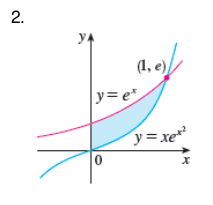
\includegraphics[width=0.5\textwidth]{problem-6-1-2.png}
        \end{center}
        \begin{proof}[Solution]
          The area $A$ is computed by
          \begin{align}
            A & = \int_0^1 e^x - xe^{x^2}\,dx  \\
              & = e-1 - \int_0^1 xe^{x^2}\,dx.
          \end{align}
          We make the substitution
          \begin{equation}
            u = x^2,
          \end{equation}
          so that
          \begin{align}
            A & = e - 1 - \frac{1}{2}\int_0^1 e^u\,du \\
              & = e - 1 - \frac{1}{2}(e - 1)          \\
              & = \frac{e-1}{2}.
          \end{align}
        \end{proof}
      \item Problem 22: Find the area bounded by $y = x^3$ and $y = x$.
        \begin{proof}[Solution]
          Sketching the two curves gives us
          \begin{center}
            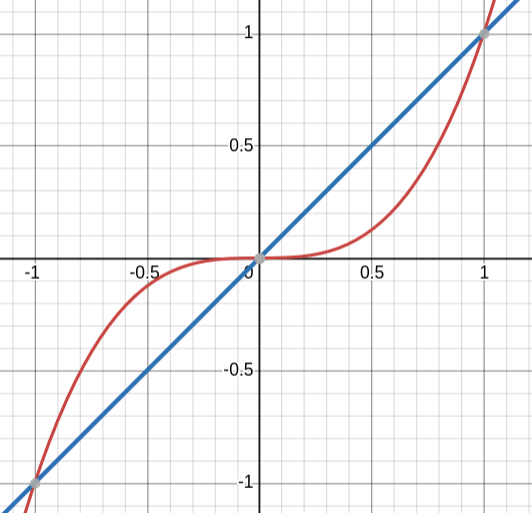
\includegraphics[width=0.5\textwidth]{problem-6-1-22.png}
          \end{center}
          Therefore, the area $A$ is computed as
          \begin{align}
            A & = \int_{-1}^0 x^3 - x \,dx + \int_0^1 x - x^3\,dx \\
              & = 2 \int_0^1 x - x^3\,dx                          \\
              & = 2\left(\frac{1}{2} - \frac{1}{4}\right)         \\
              & = \frac{1}{2}.
          \end{align}
        \end{proof}
    \end{enumerate}
\end{enumerate}
\end{document}
